\chapter{Training a Classifier Agent}

The subtraction techniques are very effective at  modeling PSF differences, nevertheless there are many defects left behind after a subtraction. This is also a well known issue in the difference image analysis. 
The bogus residual sources arise primarily from PSF mismatch and mis-alignments of the images.
Several examples of this kind are shown on figure \ref{fig:subtraction_errors}

\begin{figure}
\centering
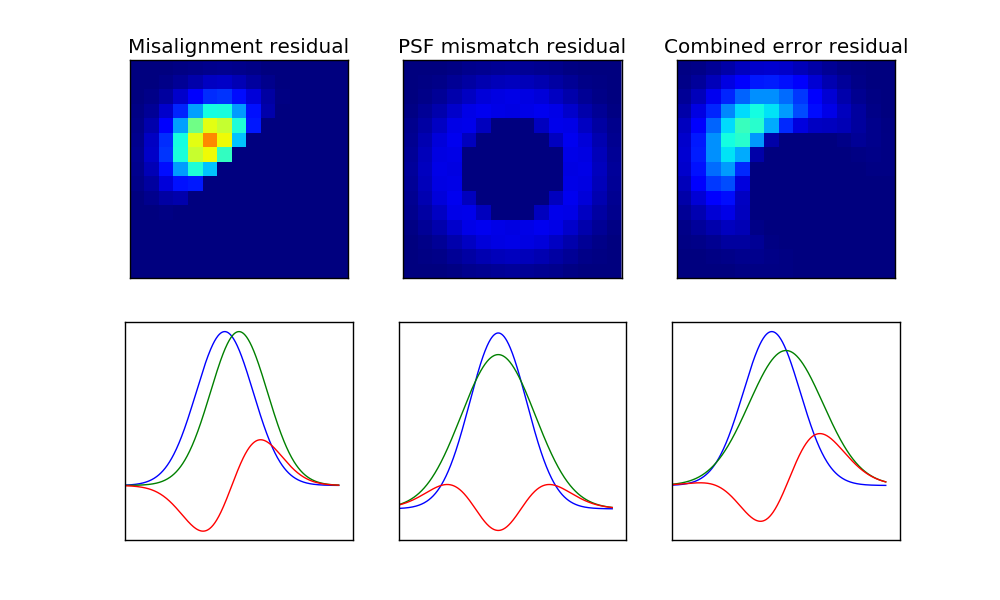
\includegraphics[scale=0.5]{figures/subtraction_error}
\caption{Some examples of subtraction errors due to misalignment and wrong PSF matching.
The top row shows typical morphology of residuals for different types of mimatches.
The bottom row shows cross sections of the top row showing the object profiles in blue and green and the subtraction in red.
First column corresponds to a displacement of the object with respect to the reference. 
The second column represents objects with different PSF.
The third column is the more typical kind of bogus residual, a combination of displacement and PSF mismatch.}
\label{fig:subtraction_errors}
\end{figure}

These defects can easily confuse algorithms of source detection like SExtractor or similar that relies on excess of flux over the background. For that, it is needed to have a computerized agent capable of discriminating bogus sources from real transients on the subtracted image. 

This is the task of a Machine Learning (ML) agent trained for that purpose. The real bogus classifier, as it is named in the literature relies on --usually morphological-- features to perform the classification.

Machine Learning is such an extensive and intensive area of research with many applications in many fields.

Since the ML field is so wide, to conduct a ML experiment one must make a few decisions. Even most importantly than the particular algorithm, 
for which there are hundreds and modifications are being published all the time, it's the data that drives the efficiency of the method.

As the saying goes:

\begin{quotation}
Big data will beat a good algorithm \textcolor{red}{Find exact quote and author}
\end{quotation}

For our main test, I decide to train a Random Forest ML algorithm on a training set developed especially for this.

The Random Forest algorithm is an `ensemble' method. Meaning it is a collection of other methods whose results will be averaged over somehow.

In this case, a Random Forest is an `ensemble' of Decision Trees. A Decision Tree is basically a tree of nodes. Each node represent a bifurcation based on one feature. The features and branching threshold on each node are chosen maximizing the expected information gain (or entropy loss) on the training set. That is, how well the bifurcation separates the training data for each class.

Random Forest bootstraps the data so that each subset of data will train a Decision Tree on a random subset of the features. After all Decision Trees are trained this way, the collection of Trees will give the final classification.

A single Decision Tree suffers of great variance, even for big amounts of data. The bifurcations on the greedy algorithm are naturally very dependent on the training set. A small variation on it may create a complete different tree. Random Forest reduces this variance by averaging over many trees. This also creates more realistic and fuzzy class boundaries on the feature space.

On the next section I explain how the training data was prepared.

\section{Training Data}

The main challenge to generate training data is the great unbalance between bogus sources due to imperfect subtraction and actual real transients.

On a typical image, the number of bogus sources can be of a hundred, and the rate of real transients can be only a handful. 

The Machine Learning problem becomes one of `Information Retrieval'. We are mainly interested in only one class, the real transients, and we need to retrieve samples of that class from a sea of bogus transients.

In a situation like that, a very unbalanced training set can bring about spurious results. As an example, imagine a training set with 90 bogus and 10 reals. The Zero Rule Classifier --that is the classifier that classifies everything as bogus-- would have a 90\% Precision and 100\% Recall for the bogus class. An unbalanced training set could also create classifiers with large variance due to the small set of real samples.

`Recall' measures the fraction of samples of the relevant class that were retrieved by the classifier out of the total number of reals in the set.
The class we are mainly interested in for the Recall is that of the real transient examples.

To generate a balanced training set with comparable amounts of reals and bogus, I generate reals by selecting sources on an image and erasing them on the reference. That way, after a subtraction, those sources will appear as transient events, that is, objects in the image that don't have a corresponding object on the reference.

The image set used for this purpose is CSTAR, but any other set will also perform similarly.

The advantage of this method, compared to other methods like injecting fake sources, is that the `transients' obtained this way will have all the particular characteristics of the CCD and instrument from the image set in which we are interested to work. It will also have the characteristics of the subtraction method imperfections, but this is not exclusive to this method.

The `bogus' set is also collected at the same time along with the `real' set.

To have equal representation of sources of different magnitudes, the sources are first binned into 10 bins of \textcolor{red}{magnitude/flux?} and taken from different regions of the CCD.
We partition the image in a 4 by 4 grid and we select one star from each region and we do so for each magnitude bin. \textcolor{red}{explain better!!!}

\subsection{The CSTAR image-set preparation}

The CSTAR image set is a high cadence set of images taken in the winter of 2010 in Antarctica, the South Pole. It comprises 6 months of data with an average cadence of \textcolor{red}{1 min ???? check}.

Since the amount of data is so large, for the purpose of training, we created a subset of 626 images, with a cadence of about an hour during the best seeing month of June (May 31st to June 30th, 2010). The subset was named `cstar\_june\_selection'. The first 10 images of this set (named cstar\_june\_01) is used for training purposes and the rest can be used to search for transients. 

The images are mostly clean, that is they were bias and flat corrected.
Nevertheless, the images suffer from `bleeding' even though they have low exposure time. This bleeding is very significative for bright stars and less so for dimmer stars but still present nonetheless.

The bled stars were covered with the median and a separate mask was created for the covered pixels for future reference. This pixel mask also includes defective pixels (dead lines and columns in the CCD).

The date-time information on the header was also updated according to \textcolor{red}{[ref]}.

For each of these images, we aligned a reference image with it using the package `astroalign' (see section astroalign) and also performed a image subtraction using the delta basis method on a 4 by 4 grid.

\section{The Classifier}

As previously said, we trained a Random Forest classifier based on 7,624 examples of fabricated transients (as described in section data) and 7,624 bogus picked at random from the subtraction images. This totals 15,248 samples for training and validation.

The features used for this classifier were selected from the popular source extractor software SExtractor [Bertin ??]. We chose the features that had relation to the morphology of the source and some other features derived from them.
The whole list is presented in table \ref{mlfeatures}.

Several scores about the performance of the classifier on the training data are condensed in the scores table (\ref{mlscores}).

\begin{table}
\centering
\begin{tabular}{|l| >{\itshape}l|}
  \hline
  x2 & Sum of the x squared values $\sum x^2 $ \\ \hline
  y2 & Sum of the y squared values $\sum y^2 $\\ \hline
  xy & Sum of the product of x and y values $\sum xy $\\ \hline
  cxx, cyy, cxy & Same as x2, y2 and xy in the convolved image  \\ \hline
  a, b, theta & semi-major axis, semi-minor axis and orientation of the best ellipse fit to the object \\ \hline
  mag\_aper & Aperture magnitude of the object in the subtraction image \\ \hline     magerr\_aper & Error of mag\_aper \\ \hline
  flux\_aper & Aperture flux in counts of the object in the subtraction image \\ \hline
  fluxerr\_aper & Error of flux\_aper \\ \hline
threshold & \\ \hline
flux\_max & Maximum value of the flux \\ \hline
fwhm & Full width at half maximum \\ \hline
deltax & Width in pixels of the object (X\_MAX - X\_MIN) \\ \hline
deltay & Height in pixels of the object (Y\_MAX - Y\_MIN) \\ \hline
ratio & $\min$(deltax, deltay)/ $\max$(deltax,deltay,1) \\ \hline
roundness & a/b\\ \hline
peak\_centroid & Distance in pixels from the pixel with highest count to the centroid of the object \\ \hline
\end{tabular}
\caption{Random Forest Features}
\label{mlfeatures}
\end{table}

\begin{table}
\centering
\begin{tabular}{| >{\itshape}l | l |}
  \hline
  accuracy & 0.9935 \\ \hline
  precision & 0.9956 \\ \hline
  recall & 0.9915 \\ \hline
  F measure & 0.9936 \\ \hline
\end{tabular}
\caption{Random Forest Scores}
\label{mlscores}
\end{table}

On the training data, the performance is quite good, with all indicators scoring above 99 percent.

In the confusion matrix (table \ref{mlconfusionmatrix}) we see that only 65 out of 7,624 of the reals were mis-classified as bogus, and only 33 bogus out of the 7,624 were mis-classified as reals. These very low numbers explain the very high performance scores of the classifier.

\begin{table}
\centering
\begin{tabular}{ l|c|c| }
\multicolumn{1}{r}{}
 &  \multicolumn{1}{c}{real}
 & \multicolumn{1}{c}{bogus} \\
\cline{2-3}
{\it Classified as} real & 7591 & 33 \\
\cline{2-3}
{\it Classified as} bogus & 65 & 7559 \\
\cline{2-3}
\end{tabular}
\caption{Confusion Matrix}
\label{mlconfusionmatrix}
\end{table}

The ROC curve is presented in figure ??.

\textcolor{red}{TO DO: Add analysis of feature importance}

\section{Testing the classifier on real data}

Once we have trained our classifier with training data, we wanted to also test it in a more real situation. For that we apply the classifier to the rest of the cstar\_june\_selection data set in search of actual transients of the image.

The Random Forest classifier will not only predict the class, but can also output a probability for that class.

Setting the probability to 0.9, the classifier returns the most likely transient events. The rate of real transient in the images is of about 15 per image for this probability threshold.

Some examples of these are shown in figure ??.

For very faint events or events that comprise very few pixels in the image, we can have additional filters that weed them out. Although, some of this could be of astronomical interest and discarding them could result in its loss.



\begin{comment}
	* Our test-drive with OIS + ML. Results of paper (hopefully)
		* Test data we used (CSTAR)
		* Processing our raw data (selecting images for a dataset, cleaning images, fixing headers, performing subtractions, identifying sources in subtractions, stamps)
		* Getting samples for training (labeling data as RB, winnow, first run of ML)
		* Feature exploration of data (SExtractor features, derived features, morphological features like Zernike, Chebyshev, Fourier, etc.)
		* Random Forest + SMOTE + Cost Matrix (how well did this perform?)
		* Is it reproducible in other data sets?
\end{comment}


